\graphicspath{{chapters/notes/01/images/}}
\chapter{Introduction}

\section{Genetics and genomics}
Genetics is the study related to specific genes and their variants with a known effect on the phenotype.
Genomics is focused on the function and structure of the human genome, evolution and anything relating to the whole genome:

\begin{multicols}{2}
	\begin{itemize}
		\item Coding regions.
		\item Non-coding regions.
		\item Linear and non-linear structures.
		\item Cell physiology and pathology.
	\end{itemize}
\end{multicols}

	\subsection{Genetics}
	Genetics is the study of heredity, or how the characteristics of living organisms are transmitted from one generation to the next via DNA.
	It dates back to Augustinian friar and scientist Gregor Mendel.
	It involves the study of a specific and limited number of genes or their part that have a known function.

	\subsection{Genomics}
	Genomics is the study of the entirety of an organism's genes, the genome.
	Using high-performance computing and mathematics techniques known as bioinformatics, genomics researchers analyse enormous amounts of DNA-sequence data to find variations that affect health, disease or drug response.
	When dealing with the human genome that means searching through about $3$ billion units of DNA across $23000$ genes.

	\subsection{Differences between genetics and genomics}
	The main difference between genomics and genetics is that genetics scrutinizes the functioning and composition of the single gene, where genomics addressees all genes and their relationships in order to identify their combined influence on the growth and development of the organism.

	\subsection{The role of computational biology}
	Computational Biology encompasses a wide range of numerical methods to analyse and integrate large scale data towards the understanding of molecular, cellular and structural biology.
	Possible studies of computational biology are:

	\begin{multicols}{2}
		\begin{itemize}
			\item Semi-quantitative simulations of metabolic pathways.
			\item 3D protein-protein interaction.
			\item Characterization of 3D chromatic structure,
			\item Discovery and characterization of disease related variants.
		\end{itemize}
	\end{multicols}

	The main subjects involved are:

	\begin{multicols}{3}
		\begin{itemize}
			\item Biology.
			\item Genetics.
			\item Statistics.
			\item Calculus.
			\item Computer science.
			\item Bioinformatics.
		\end{itemize}
	\end{multicols}

	The focus of this work is on hot to mine raw data, mainly from sequencing, how to exploit it for quality control (QC) and hot to interpret the obtained results in the context of human diseases, especially in cancer.


\section{Basis of human genomics}
The genetic make-up is different in all human it is responsible for our diversity.
SNPs (single nucleotide polymorphisms) and CNVs (copy number variants) contribute to make us different.
The majority of the external phenotypes come from genetic variance that are inherited or, in minor measure, acquired.

	\subsection{Single nucleotide polymorphisms}
	Single nucleotide polymorphisms or SNPs are changes of one nucleotide in the sequence of a gene.
	They constitute $1\%$ of the difference between two unrelated individuals' genomes and they can be used as quality control assets.

	\subsection{Copy number variants}
	Copy number variants or CNVs are the differences in number of alleles for a gene present in one individual.
	They contribute much more than SNPs in the difference between unrelated individuals, but they're less known as inherited variants, as they are harder to quantify and detect.
	CNV are distinguished as gain-CNV (where the number of alleles is greater than two) and loss-CNV (where the number of alleles is $2$, $1$, or $0$).
	It is of note that if both parents have only one copy of a gene their child can have none.
	CNV span $\gg1\%$ difference between two unrelated individual genomes.

	\subsection{Inherited variants}
	Inherited variants can be characterized by penetrance and allele frequency.

	\begin{figure}[H]
		\centering
		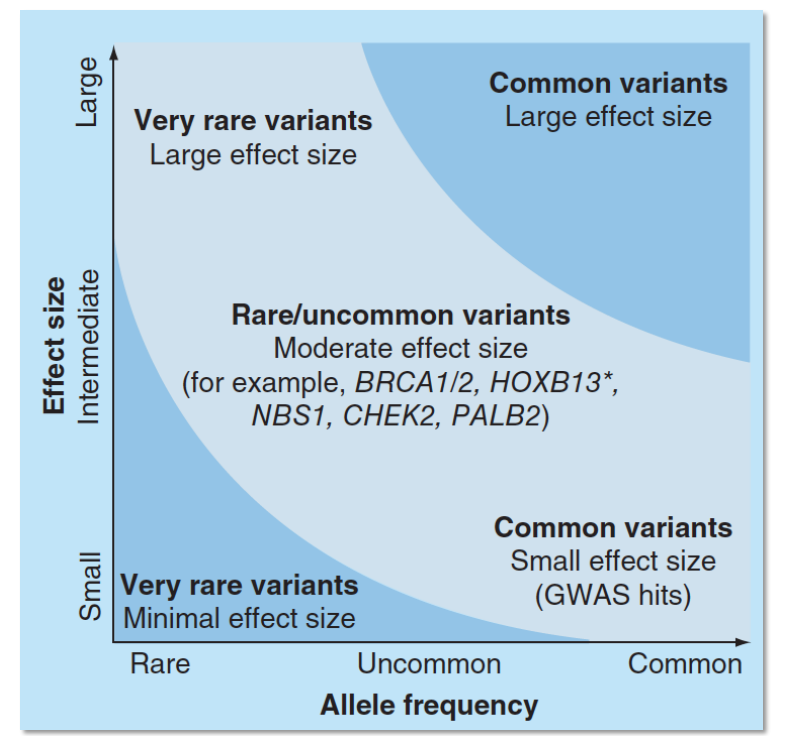
\includegraphics[width=0.5\textwidth]{relevance.png}
		\caption{R. Eeles, Future Sci. OA (2016) 2(1), FSO87. Review on prostate cancer.\\
			\textbf{Common SNPs}: $\frac{1}{4}$ of individual is homozygous for A1, $\frac{1}{4}$ is homozygous for A2, $\frac{1}{2}$ is heterozygous. The minor allele frequency is around 30-50\% with low penetrance.\\
			\textbf{Rare SNPs}: typically have very large size effect: if they are related to very specific traits they will have high penetrance. They constitute deleterious variants.}
		\label{fig:relevance}
	\end{figure}

		\subsubsection{Penetrance}
		Penetrance is the proportion of individuals carrying an allele (or genotype) that also expresses the trait (or phenotype) associated with it.

		\subsubsection{Allele frequency}
		Allele frequency is the ratio between the number of times the allele of interest is observed in a population over the total number of copies of all the alleles at that particular genetic locus in the population:

		$$AF = \frac{\# allele\ of\ interest}{\# copies\ of\ all\ the alleles\ at\ the\ genetic\ locus}$$

		Recent studies have shown that genetic variance contributes to predisposition to certain diseases.
		It is also emerging that rare pathogenic variants tend to have an high penetrance.
		This means that if a variant is pathogenic and rare, it's probable that all patients affected by the disease carry that particular mutation.
		This is represented by the top part of the diagram shown in figure \ref{fig:relevance}.
		On the other hand, common variants could be associated to predisposition or susceptibility to the disease with low penetrance.
		In the middle on the diagram well-known variants correlated to cancer are found.
		The majority of these have a moderate size effect: not everyone who has the variation develops the disease.

		\subsubsection{Differences in Genetic Make-Up, an example}
		One example of how the genetic make-up plays a role in disease is the ADME genes.
		ADME stands for \textit{Absorption, distribution, metabolism and elimination}.
		It is a set of genetic variants that is able to change the ability of the organism to react to certain compounds causing pharmacokinetic variability and influencing the patient's treatment response.
		Both common and rare variants are involved.
		Figure \ref{fig:adme} represent a subset of them.

		\begin{figure}[H]
			\centering
			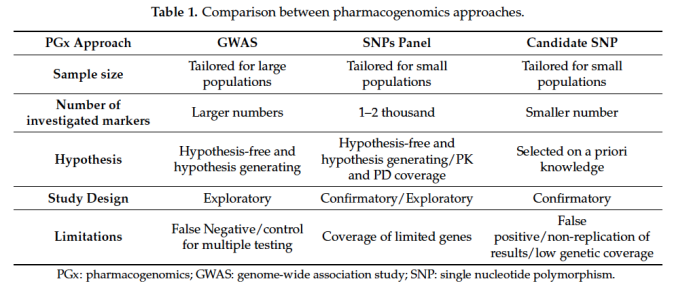
\includegraphics[width=0.7\textwidth]{ADME.png}
			\caption{From review: \textit{Pharmacogenomic Profiling of ADME Gene Variants: Current Challenges and Validation Perspectives}}
			\label{fig:adme}
		\end{figure}

		A therapeutic approach that considers these variations could be very useful in precision medicine.

	\subsection{Somatic Variants}
	Somatic variants are \textbf{not} inherited from parents and are not transmitted to offspring.
	Most of them, but not all, are harmless.
	They can also be present in only a subset of the cells in an individual.

		\subsubsection{Classification}
		Somatic variants can be classified as:

		\begin{multicols}{2}
			\begin{itemize}
				\item Single Nucleotide Variants (SNV).
					SNVs are a single point mutation restricted to a certain population of cells in an individual.
				\item Indels few nucleotides deletions.
				\item Rearrangements, like gene translocation, chromosome breakage and chromothripsis (which falls in the subcategory of chromosomal rearrangements).
				\item Somatic Copy Number Aberrations (SCNA).
			\end{itemize}
		\end{multicols}


		\subsubsection{Types of acquired DNA aberrations}

			\paragraph{Translocation}
			Translocation happens when a sequence is moved from one genetic locus to another.
			It can be:

			\begin{multicols}{2}
				\begin{itemize}
					\item Balanced: two sequences exchange locus and the overall quantity of DNA is maintained.
					\item Unbalanced: only one sequence move, generating an insertion.
				\end{itemize}
			\end{multicols}

			\paragraph{Inversion}
			Inversion happens when a sequence inverts its orientation.
			This aberration involves only one chromosome.
			The sequence of the inversion doesn't change, and the event will only be detected at its head and tail.

			\paragraph{Copy number changes}
			Copy number changes are events in which the quantity of DNA changes.
			They could involve one or more chromosomes.
			They can be:

			\begin{multicols}{2}
				\begin{itemize}
					\item Duplication: a sequence doubles its copy number.
					\item Deletion: a sequence is lost.
				\end{itemize}
			\end{multicols}

			\paragraph{Chromoplexy}
			Chromoplexy derives from the Greek \textit{pleko}, meaning to weave, or to braid.
			It describes a class of complex somatic DNA rearrangements whereby abundant DNA deletions and intra- and inter-chromosomal translocations that have originated in an interdependent way occur within a single cell cycle.

			\paragraph*{Chromothripsis}
			Chromothripsis derives from the Greek \textit{thripsis}, meaning shattering into pieces.
			It describes a clustered chromosomal rearrangement in confined genomic regions that results from a single catastrophic event, usually limited to one chromosome.

			\paragraph*{Kataegis}
			Kataegis derives from the Greek kataigis, meaning thunder.
			It describes a phenomenon that is characterized by large clusters of mutations (hypermutation) in the genome of cancer cells.
			An APOBEC family enzyme might be responsible for the kataegis process.

\section{Experimental techniques to detect variants/aberrations}

	\subsection{Karyotyping}
	Karyotyping is the process of pairing and ordering all the chromosome of an organism, providing a genome-wide snapshot of an individual's chromosomes.
	This experiment was used to try and detect genomic aberration, but it proved inadequate because its resolution wasn't enough.
	In particular it missed all sequence specific variants, breakpoints that could not be detected until the development of NGS.

	\subsection{Sequence capture for cancer genomics}
	In the paper summarized in \ref{ch:Meyerson} it is described a typical sequence capture for cancer genomics.

		\subsubsection{Reference}
		After sequencing there is a need to align the reads to a reference genome.
		This is especially needed when studying somatic changes.
		The best reference for this king of studies is the individual's own genome, usually retrieved from white blood samples.
		Both cancer and normal DNA can be aligned to detect if an aberration is cancer specific or is present in both normal and cancer DNA.
		The \textbf{match normal} tool is used to distinguish SNV from rare SNPs, somatic and germline indels, but also to make sure that copy number variations are somatic.
		Baits are nowadays used in the sequencing step, in order to sequence only the exome or specific part of the genome, as to make the sequencing process more cheap.

		\subsubsection{Deepness}
		Another fundamental parameter in sequencing is the deepness.
		A more deep sequencing is needed to find subclonal event that could increase cancers' fitness, like the ability to escape the immune system.
		It is necessary because not all cells present all the mutations characterizing the subclonal event and because the purity of a tumour sample is not always optimal.


		\subsubsection{Single End (SE) and Paired End (PE) reads} \label{SE_PE}

			\paragraph{Single end sequencing}
			Single-read sequencing involves sequencing DNA from only one end.
			This solution delivers large volumes of high-quality data, rapidly and economically.

			\paragraph{Paired end sequencing}
			Paired-end sequencing allow to sequence both ends of a fragment and generate high-quality alignable data.
			It facilitates the detection of genomic rearrangements and repetitive sequence elements, as well as gene fusions and novel transcripts while providing double the coverage as a single-end protocol.
			It gives important information of the relative position of a molecule with respect to the reference, and is a necessary choice when structural aberration need to be assessed.
			This protocol is however twice as expensive as the single-end one.

			\paragraph{Ability of paired end sequencing to detect genomic aberrations}
			Figure \ref{fig:igv} gives a nice graphical overview of genomic aberrations detectable by NGS, especially using PE sequencing.
			In particular the traslocation breakpoint in figure \ref{fig:igv} would not be detectable without paired end sequencing.
			The most important parameter when studying deletions and insertion is to have enough coverage to perform significant downstream analysis, besides structural informations.

			\begin{figure}[H]
					\centering
					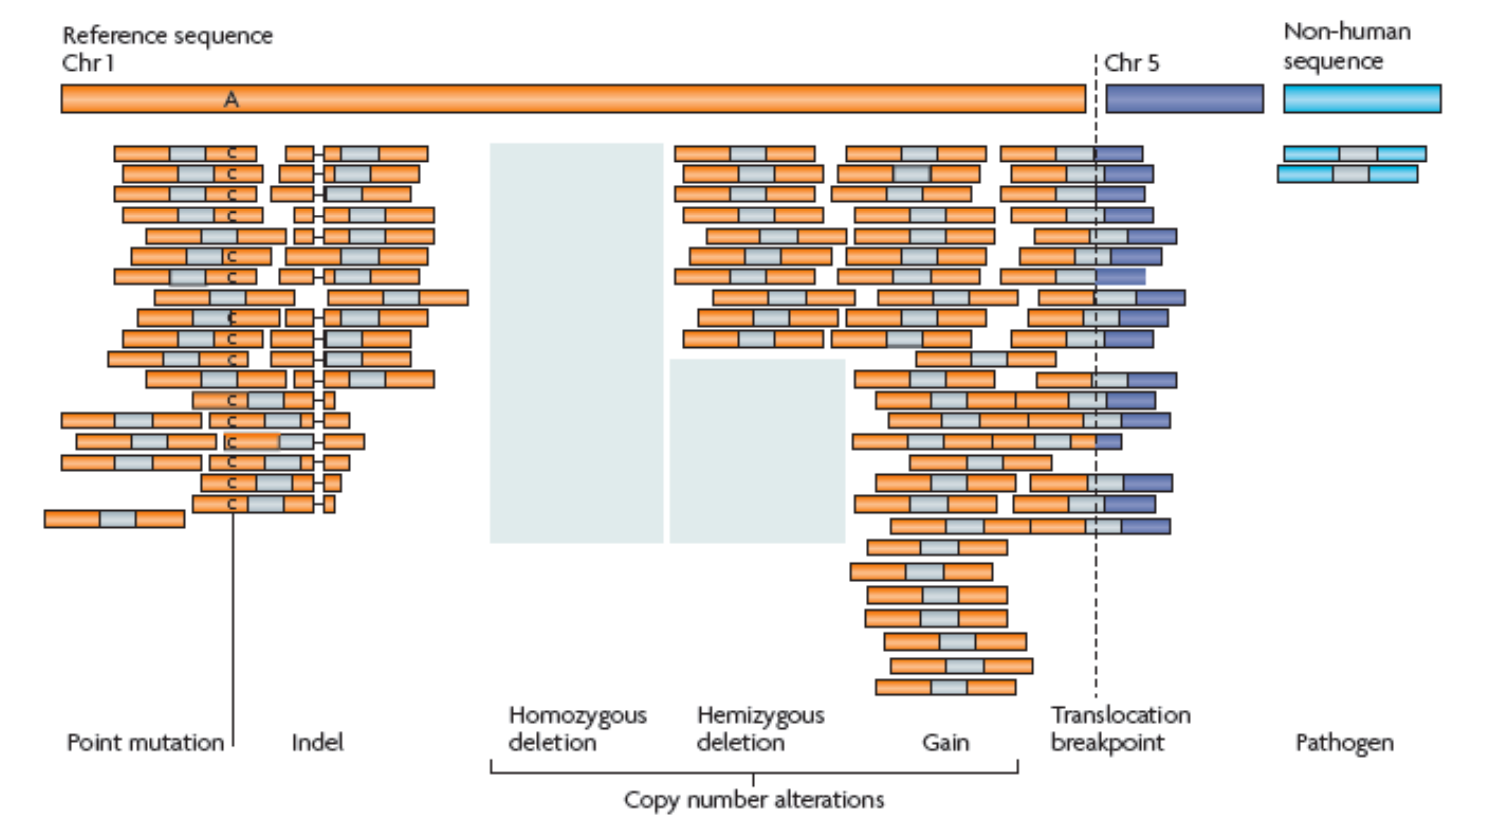
\includegraphics[width=0.7\textwidth]{igv.png}
					\caption{\textit{Advances in understanding cancer genomes through second-generation sequencing}, Meyerson et al., Nature Reviews Genetics 2010}
					\label{fig:igv}
			\end{figure}
